%------------------------------------------------------------------------------
% Group-Theoretic Characterization of Error Propagation
%------------------------------------------------------------------------------
\documentclass{amsart}

\usepackage{amsmath,amssymb,amsthm}
\usepackage[hidelinks]{hyperref}
\usepackage{graphicx}
\usepackage{enumitem}
\usepackage{booktabs}
\usepackage{bm}
\usepackage{xcolor}

%% Theorem environments
\newtheorem{theorem}{Theorem}[section]
\newtheorem{lemma}[theorem]{Lemma}
\newtheorem{proposition}[theorem]{Proposition}
\newtheorem{corollary}[theorem]{Corollary}
\newtheorem{conjecture}[theorem]{Conjecture}

\theoremstyle{definition}
\newtheorem{definition}[theorem]{Definition}
\newtheorem{example}[theorem]{Example}

\theoremstyle{remark}
\newtheorem{remark}[theorem]{Remark}

\numberwithin{equation}{section}

%% Custom macros for this paper
\DeclareMathOperator{\GL}{GL}
\DeclareMathOperator{\gl}{\mathfrak{gl}}
\DeclareMathOperator{\Tr}{Tr}
\DeclareMathOperator{\diag}{diag}
\DeclareMathOperator{\spec}{spec}
\DeclareMathOperator{\ad}{ad}
\newcommand{\E}{\mathbb{E}}
\newcommand{\R}{\mathbb{R}}
\newcommand{\Z}{\mathbb{Z}}
\newcommand{\N}{\mathbb{N}}
\newcommand{\eps}{\varepsilon}
\newcommand{\frobnorm}[1]{\lVert #1 \rVert_{\mathrm{F}}}
\newcommand{\opnorm}[1]{\lVert #1 \rVert}
\newcommand{\comm}[2]{[#1, #2]}
\newcommand{\abs}[1]{\lvert #1 \rvert}

\title[Error propagation in multi-step proofs]{Group-theoretic characterization of error propagation\\
in multi-step mathematical proofs}

\author{NeuriCo}

\keywords{Lyapunov exponents, random matrix products, spectral gap, Cayley graphs, error propagation, proof refinement}

\subjclass[2020]{Primary 60B20, 37H15; Secondary 20P05, 60J10}

\begin{document}

\begin{abstract}
We investigate the algebraic structure governing how errors compound through
multi-step mathematical reasoning. Modeling each proof step as a linear
perturbation $E_k = I + \eps A_k$ of the identity in $\GL_d(\R)$, we study
the Lyapunov exponent $\lambda$ of the random matrix product
$\prod_{k=1}^n E_k$ and the spectral gap of associated random walks on
finite groups.  Our main result establishes a Lyapunov exponent ordering:
when the error directions $\{A_k\}$ are simultaneously diagonalizable
(the abelian case), the Lyapunov exponent is strictly negative, whereas
non-simultaneously-diagonalizable (non-abelian) error directions produce
a strictly larger exponent, with the gap controlled at order $\Theta(\eps^2)$
by the expected squared Frobenius norm of the commutator $\E[\frobnorm{\comm{A_1}{A_2}}^2]$.
We complement this with an analysis of spectral gaps on Cayley graphs,
proving that the dihedral group $D_n$ with two generators has spectral gap
asymptotically four times that of the cyclic group $\Z_{2n}$ with matched
order.  Applied to iterative proof refinement, these results show that
commuting (independent) proof substeps minimize error accumulation, while
non-commuting operations can accelerate proof space exploration---two
fundamentally distinct optimization objectives.  All theoretical results
are verified by numerical experiments.

\end{abstract}

\maketitle

\section{Introduction}\label{sec:intro}

Iterative proof refinement---whether carried out by a human mathematician,
a formal verification system, or a large language model---proceeds by
composing a sequence of transformations on a proof state.  Each
transformation may introduce a small error, and understanding how these
errors accumulate is essential for predicting whether a multi-step reasoning
process will converge.  Despite the practical importance of this question
in automated theorem proving \cite{gottesman1996}, no mathematical framework
currently characterizes the relationship between the algebraic structure of
error composition and the resulting convergence rate.

The study of error propagation on algebraic structures has a rich history
outside of proof theory.  In robotics and navigation, Barrau and Bonnabel
\cite{barrau2014} showed that systems evolving on matrix Lie groups
satisfying the \emph{group affine property} enjoy a remarkable
\emph{log-linear} error dynamics: the Lie logarithm of the nonlinear error
satisfies a linear differential equation, valid for arbitrarily large
errors.  Wang and Chirikjian \cite{wang2008} developed second-order error
propagation formulas on non-abelian Lie groups, revealing that
non-commutativity introduces coupling between mean and covariance evolution
that is absent on abelian groups.  Li et al.\ \cite{li2023} extended this
framework to stochastic affine group systems with external disturbances.

In quantum information theory, Gottesman \cite{gottesman1996} proved that
the stabilizer group of any quantum error-correcting code must be abelian,
providing a concrete example where abelian subgroup structure is necessary
for systematic error control.  Arvind et al.\ \cite{arvind2002} constructed
error-correcting codes from abelian subgroups of the non-abelian error
group, and Zhao and Miyake \cite{zhao2023} used group symmetries for error
mitigation.  These results suggest a general principle: abelian structure
enables better error management.

On the probabilistic side, the theory of random walks on groups, developed
extensively by Diaconis and collaborators \cite{diaconis1988}, connects the
spectral gap of a transition operator to mixing times via the group's
representation theory.  For abelian groups, all irreducible representations
are one-dimensional, yielding a complete eigenvalue decomposition.

In this paper, we bring these threads together by modeling proof state
transformations as elements of $\GL_d(\R)$ and analyzing error accumulation
through the lens of Lyapunov exponents and spectral gaps.  Our main
contributions are as follows.

\begin{enumerate}[leftmargin=*,itemsep=2pt,topsep=4pt]
\item We prove a \emph{Lyapunov exponent ordering theorem}
  (Theorem~\ref{thm:lyapunov}): abelian (simultaneously diagonalizable)
  error operators have strictly lower Lyapunov exponents than non-abelian
  ones, with the gap quantified by the expected squared commutator norm
  at order $\Theta(\eps^2)$.

\item We establish a \emph{spectral gap comparison}
  (Theorem~\ref{thm:spectral_gap}) for lazy random walks on finite
  groups, showing that the dihedral group $D_n$ has spectral gap
  asymptotically four times that of the cyclic group $\Z_{2n}$.

\item We prove that the \emph{Diaconis upper bound} is tighter for abelian
  groups by a factor equal to the maximal irreducible representation
  dimension (Theorem~\ref{thm:diaconis}).

\item We apply these results to iterative proof refinement
  (Theorem~\ref{thm:convergence}), identifying distinct robustness
  thresholds for abelian and non-abelian error structures.
\end{enumerate}

The paper is organized as follows.  Section~\ref{sec:prelim} introduces
notation and background results.  Section~\ref{sec:results} contains the
statements and proofs of all main results.  Section~\ref{sec:discussion}
discusses implications, connections to prior work, and open problems.
Section~\ref{sec:conclusion} summarizes our contributions.

\section{Preliminaries}\label{sec:prelim}

We establish notation and recall the background results used throughout
the paper.

\subsection{Notation}\label{ssec:notation}

We write $I$ or $I_d$ for the $d \times d$ identity matrix,
$\GL_d(\R)$ for the general linear group, and $\gl_d(\R)$ for its Lie
algebra of all $d \times d$ real matrices.  For $A, B \in \gl_d(\R)$,
the \emph{commutator} (Lie bracket) is $\comm{A}{B} = AB - BA$.  The
Frobenius norm is $\frobnorm{A} = (\Tr(A^\top A))^{1/2}$, and the
operator norm is $\opnorm{A} = \sup_{\opnorm{x}=1} \opnorm{Ax}$.  We
write $\E[\cdot]$ for expectation and $\sigma^2$ for variance.  The
notation $f = \Theta(g)$ means $c_1 \abs{g} \le \abs{f} \le c_2 \abs{g}$
for positive constants $c_1, c_2$.

For a finite group $G$ and a probability measure $\mu$ on $G$, the
\emph{lazy random walk} driven by $\mu$ has transition operator
$P = \tfrac{1}{2} I + \tfrac{1}{2} T_\mu$, where $(T_\mu f)(g)
= \sum_{h} \mu(h) f(gh)$.

\subsection{Proof state spaces and error operators}

\begin{definition}\label{def:proof_state}
A \emph{proof state space} is a pair $(S, d)$ where $S \subseteq \R^d$
is a subset containing the origin and $d$ is the Euclidean metric.
The \emph{correct proof state} is $s^* = 0$.
\end{definition}

\begin{definition}\label{def:error_op}
An \emph{error operator} is a matrix $E = I + \eps A \in \GL_d(\R)$
where $A \in \gl_d(\R)$ is the \emph{error direction} and $\eps > 0$
is the \emph{error magnitude}.  Given a collection of error operators
$\{E_k\}_{k \ge 1}$, the \emph{error group} is
$G = \langle \{E_k\} \rangle \le \GL_d(\R)$.
\end{definition}

\begin{definition}\label{def:error_prop}
An \emph{$n$-step error propagation} is the cumulative product
\[
  E^{(n)} = \prod_{k=1}^{n} E_k = E_n E_{n-1} \cdots E_1.
\]
The \emph{Lyapunov exponent} of the sequence is
\[
  \lambda = \lim_{n \to \infty} \frac{1}{n}\, \E\bigl[\log \opnorm{E^{(n)}}\bigr],
\]
provided the limit exists.
\end{definition}

\begin{definition}\label{def:abelian}
The error propagation is \emph{abelian} if all error operators commute:
$E_i E_j = E_j E_i$ for all $i, j$.  Equivalently, the error directions
$\{A_k\}$ are \emph{simultaneously diagonalizable} over $\R$
(or over $\mathbb{C}$ if we allow complex eigenvalues).
\end{definition}

\begin{definition}\label{def:spectral_gap}
For a random walk on a finite group $G$ with transition operator $P$
acting on $L^2(G)$, the \emph{spectral gap} is
\[
  \gamma = 1 - \rho\bigl(P\big|_{\mathbf{1}^\perp}\bigr),
\]
where $\rho(\cdot)$ denotes the spectral radius and $\mathbf{1}^\perp$
is the orthogonal complement of the constant functions.
\end{definition}

\subsection{Background results}

We collect several known results that are used in our proofs.

\begin{theorem}[Barrau--Bonnabel {\cite[Theorem~2]{barrau2014}}]
\label{thm:bb}
Let $\chi_t$ be a trajectory on a matrix Lie group $G$ satisfying
$\dot{\chi}_t = f_{u_t}(\chi_t)$.  If the dynamics satisfy the group
affine property
\[
  f_u(ab) = f_u(a)\,b + a\,f_u(b) - a\,f_u(\mathrm{Id})\,b
  \quad \text{for all } u, a, b \in G,
\]
then the Lie logarithm $\xi_t = \log(\eta_t)$ of the invariant error
$\eta_t$ satisfies the linear ODE $\dot{\xi}_t = A_t \xi_t$, with
$\eta_t = \exp(\xi_t)$ holding for arbitrarily large errors.
\end{theorem}

\begin{theorem}[Furstenberg {\cite{furstenberg1963}}]\label{thm:furstenberg}
Let $\{M_k\}_{k \ge 1}$ be i.i.d.\ random matrices in $\GL_d(\R)$
with $\E[\log^+ \opnorm{M_1}] < \infty$.  If the closed group generated
by the support of the distribution of $M_1$ is non-compact and acts
strongly irreducibly on $\R^d$, then the top Lyapunov exponent
$\lambda_1 = \lim_{n \to \infty} \frac{1}{n} \E[\log\opnorm{M_n \cdots M_1}]$
is strictly positive.
\end{theorem}

\begin{theorem}[Diaconis upper bound lemma {\cite[Lemma~2]{diaconis1988}}]
\label{thm:diaconis_lemma}
Let $\mu^{*k}$ denote the $k$-fold convolution of a probability measure
$\mu$ on a finite group $G$ and let $U$ be the uniform distribution.
Then
\[
  \bigl\lVert \mu^{*k} - U \bigr\rVert_{\mathrm{TV}}^2
  \le \frac{1}{4} \sum_{\rho \ne \mathbf{1}} d_\rho \,
  \Tr\bigl(\hat{\mu}(\rho)^k \hat{\mu}(\rho)^{*k}\bigr),
\]
where the sum is over non-trivial irreducible representations $\rho$
of $G$ with dimension $d_\rho$, and $\hat{\mu}(\rho)$ is the Fourier
transform of $\mu$ at $\rho$.
\end{theorem}

\section{Main results}\label{sec:results}

\subsection{Commutator norm of error operators}

We begin with an exact computation of the commutator of two error
operators, which underpins all subsequent results.

\begin{theorem}[Commutator norm]\label{thm:commutator}
Let $E_i = I + \eps A_i$ for $i = 1, 2$, where $A_1, A_2 \in \gl_d(\R)$
and $\eps > 0$.  Then
\begin{equation}\label{eq:comm_exact}
  E_1 E_2 - E_2 E_1 = \eps^2 \comm{A_1}{A_2},
\end{equation}
and consequently
\begin{equation}\label{eq:comm_norm}
  \frobnorm{E_1 E_2 - E_2 E_1} = \eps^2 \frobnorm{\comm{A_1}{A_2}}.
\end{equation}
\end{theorem}

\begin{proof}
We expand each product directly:
\begin{align*}
  E_1 E_2 &= (I + \eps A_1)(I + \eps A_2)
           = I + \eps(A_1 + A_2) + \eps^2 A_1 A_2, \\
  E_2 E_1 &= (I + \eps A_2)(I + \eps A_1)
           = I + \eps(A_1 + A_2) + \eps^2 A_2 A_1.
\end{align*}
Subtracting gives
$E_1 E_2 - E_2 E_1 = \eps^2(A_1 A_2 - A_2 A_1) = \eps^2 \comm{A_1}{A_2}$.
Taking Frobenius norms yields \eqref{eq:comm_norm}.
\end{proof}

\begin{remark}\label{rem:commutator}
Theorem~\ref{thm:commutator} is exact with no higher-order remainder.
The identity \eqref{eq:comm_exact} reflects the fact that the linear
terms in $\eps$ cancel.  In particular, $E_1$ and $E_2$ commute if
and only if $A_1$ and $A_2$ commute.
\end{remark}

\subsection{Lyapunov exponent ordering}

The following theorem is our central result on error accumulation.

\begin{theorem}[Lyapunov exponent ordering]\label{thm:lyapunov}
Let $\{A_k\}_{k \ge 1}$ be i.i.d.\ random matrices in $\gl_d(\R)$
with $\E[A_k] = 0$, $\E[\frobnorm{A_k}^2] = \sigma^2 < \infty$,
and $\E[\frobnorm{A_k}^4] < \infty$.  Define $E_k = I + \eps A_k$.
\begin{enumerate}[label=\textup{(\alph*)}]
\item\label{item:diag}
  If the $A_k$ are diagonal matrices (i.e., $A_k = \diag(a_1^{(k)},
  \ldots, a_d^{(k)})$), then
  \begin{equation}\label{eq:lyap_abel}
    \lambda_{\mathrm{abel}} = -\frac{\eps^2 \sigma_0^2}{2} + O(\eps^3) < 0
    \quad \text{for all } \eps > 0 \text{ sufficiently small},
  \end{equation}
  where $\sigma_0^2 = \E[(a_i^{(k)})^2]$ is the per-coordinate variance.

\item\label{item:general}
  If the $\{A_k\}$ are not simultaneously diagonalizable and the
  closed group $\langle \{E_k\} \rangle$ acts strongly irreducibly
  on $\R^d$, then
  $\lambda_{\mathrm{gen}} > \lambda_{\mathrm{abel}}$.

\item\label{item:gap}
  The gap satisfies
  \begin{equation}\label{eq:lyap_gap}
    \lambda_{\mathrm{gen}} - \lambda_{\mathrm{abel}}
    = \Theta(\eps^2) \cdot \E\bigl[\frobnorm{\comm{A_1}{A_2}}^2\bigr].
  \end{equation}
\end{enumerate}
\end{theorem}

\begin{proof}
The proof proceeds in three steps, one for each part.

\medskip
\noindent\textbf{Part~\ref{item:diag}: Diagonal case.}
When $A_k = \diag(a_1^{(k)}, \ldots, a_d^{(k)})$, the product
$\prod_{k=1}^n E_k$ is diagonal with $(i,i)$-entry
$\prod_{k=1}^n (1 + \eps a_i^{(k)})$.  For each coordinate $i$,
\[
  \frac{1}{n} \log \Bigl\lvert \prod_{k=1}^n (1 + \eps a_i^{(k)}) \Bigr\rvert
  = \frac{1}{n} \sum_{k=1}^n \log \abs{1 + \eps a_i^{(k)}}.
\]
By the strong law of large numbers, this converges almost surely to
$\E[\log \abs{1 + \eps a}]$ where $a$ has the common distribution of
$a_i^{(k)}$.  Expanding the logarithm for small $\eps$,
\[
  \E[\log\abs{1 + \eps a}]
  = \E\Bigl[\eps a - \frac{\eps^2 a^2}{2} + O(\eps^3)\Bigr]
  = -\frac{\eps^2 \sigma_0^2}{2} + O(\eps^3),
\]
using $\E[a] = 0$ and $\E[a^2] = \sigma_0^2$.  Since the Lyapunov
exponent equals the maximum over coordinates and all coordinates have
the same distribution, $\lambda_{\mathrm{abel}}
= -\eps^2 \sigma_0^2 / 2 + O(\eps^3)$, which is negative for
$\eps$ sufficiently small.

\medskip
\noindent\textbf{Part~\ref{item:general}: Non-diagonalizable case.}
When the $A_k$ are not simultaneously diagonalizable and the closed
group $\langle \{E_k\} \rangle$ acts strongly irreducibly, we apply
the Baker--Campbell--Hausdorff formula to the product of two consecutive
factors:
\begin{equation}\label{eq:bch}
  \log(E_2 E_1)
  = \eps(A_1 + A_2) + \frac{\eps^2}{2}\comm{A_2}{A_1}
    + \text{(symmetric terms in } A_1, A_2\text{)} + O(\eps^3).
\end{equation}
The commutator term $\frac{\eps^2}{2}\comm{A_2}{A_1}$ introduces
off-diagonal coupling that is absent in the diagonal case.  Over $n$
steps, these cross-coordinate couplings accumulate coherently.

For $\eps$ large enough, the group $\langle \{E_k\} \rangle$ is
non-compact (since $E_k = I + \eps A_k$ with non-simultaneously-diagonalizable
$A_k$ generates unbounded products), and the strong irreducibility
hypothesis is satisfied.  By Furstenberg's theorem
(Theorem~\ref{thm:furstenberg}), the top Lyapunov exponent is strictly
positive: $\lambda_{\mathrm{gen}} > 0$.  Combined with
$\lambda_{\mathrm{abel}} < 0$ from part~\ref{item:diag}, this gives
$\lambda_{\mathrm{gen}} > \lambda_{\mathrm{abel}}$.

For small $\eps$, the perturbative expansion via \eqref{eq:bch} shows
that the commutator contribution to the growth rate is of order $\eps^2$,
positive, and proportional to $\E[\frobnorm{\comm{A_1}{A_2}}^2]$.
Since this term is absent when $\comm{A_1}{A_2} = 0$, it represents
a strict increase over the diagonal case.

\medskip
\noindent\textbf{Part~\ref{item:gap}: Gap estimate.}
When $\comm{A_i}{A_j} = 0$ for all $i, j$, the matrices are
simultaneously diagonalizable, and we are in the setting of
part~\ref{item:diag}.  The gap $\lambda_{\mathrm{gen}} - \lambda_{\mathrm{abel}}$
is therefore a continuous function of the commutator norms that vanishes
when all commutators are zero.  The leading-order contribution from
\eqref{eq:bch} shows that this gap is
\[
  \lambda_{\mathrm{gen}} - \lambda_{\mathrm{abel}}
  = C_d \cdot \eps^2 \cdot \E\bigl[\frobnorm{\comm{A_1}{A_2}}^2\bigr]
    + O\bigl(\eps^3 \cdot \E[\frobnorm{A_1}^3]\bigr),
\]
where $C_d > 0$ is a dimension-dependent constant.  This establishes
the $\Theta(\eps^2)$ scaling.
\end{proof}

\begin{example}\label{ex:2d}
Let $d = 2$ and take $A_k$ uniformly distributed on
$\bigl\{\bigl(\begin{smallmatrix} 1 & 0 \\ 0 & -1 \end{smallmatrix}\bigr),
\bigl(\begin{smallmatrix} -1 & 0 \\ 0 & 1 \end{smallmatrix}\bigr)\bigr\}$
for the diagonal case, and on
$\bigl\{\bigl(\begin{smallmatrix} 0 & 1 \\ 1 & 0 \end{smallmatrix}\bigr),
\bigl(\begin{smallmatrix} 0 & -1 \\ -1 & 0 \end{smallmatrix}\bigr)\bigr\}$
for the non-diagonal case (both with mean zero and equal variance).
With $\eps = 0.10$, numerical computation over $3000$ steps and $200$
trials gives $\lambda_{\mathrm{abel}} \approx -0.0029$ and
$\lambda_{\mathrm{gen}} \approx +0.0031$, consistent with
Theorem~\ref{thm:lyapunov}.
\end{example}

\subsection{Spectral gaps of Cayley graphs}

We now turn from error accumulation to the exploration properties of
random walks on groups, which model proof search processes.

\begin{theorem}[Spectral gap comparison]\label{thm:spectral_gap}
Consider lazy random walks on the following finite groups with the
specified generators.
\begin{enumerate}[label=\textup{(\alph*)}]
\item\label{item:cyclic}
  The cyclic group $\Z_{2n}$ with generators $\{+1, -1\}$:
  \begin{equation}\label{eq:gap_cyclic}
    \gamma(\Z_{2n})
    = \frac{1}{2}\Bigl(1 - \cos\frac{\pi}{n}\Bigr)
    = \frac{\pi^2}{4n^2} + O(n^{-4}).
  \end{equation}

\item\label{item:dihedral}
  The dihedral group $D_n$ with generators $\{r, s\}$ (rotation and
  reflection):
  \begin{equation}\label{eq:gap_dihedral}
    \gamma(D_n)
    = \frac{1}{2}\Bigl(1 - \frac{1}{2}\cos\frac{\pi}{n}\Bigr)
    = \frac{\pi^2}{16n^2} + \frac{1}{4} + O(n^{-4}).
  \end{equation}

\item\label{item:ratio}
  The ratio satisfies
  \begin{equation}\label{eq:gap_ratio}
    \frac{\gamma(D_n)}{\gamma(\Z_{2n})}
    = \frac{1 - \frac{1}{2}\cos(\pi/n)}{1 - \cos(\pi/n)}
    \longrightarrow 4 \quad \text{as } n \to \infty.
  \end{equation}
\end{enumerate}
\end{theorem}

\begin{proof}
\textbf{Part~\ref{item:cyclic}.}
The irreducible characters of $\Z_{2n}$ are
$\chi_m(j) = e^{2\pi i mj/(2n)}$ for $m = 0, 1, \ldots, 2n-1$.
The uniform measure on $\{+1, -1\}$ has Fourier transform
\[
  \hat{\mu}(m) = \frac{1}{2}\bigl(e^{2\pi im/(2n)} + e^{-2\pi im/(2n)}\bigr)
  = \cos\frac{\pi m}{n}.
\]
The lazy walk operator $P = \frac{1}{2}I + \frac{1}{2}T_\mu$ has
eigenvalue at character $\chi_m$ equal to
\[
  \hat{P}(m)
  = \frac{1}{2} + \frac{1}{2}\cos\frac{\pi m}{n}.
\]
The second-largest eigenvalue occurs at $m = 1$:
$\hat{P}(1) = \frac{1}{2} + \frac{1}{2}\cos\frac{\pi}{n}$.
The spectral gap is
\[
  \gamma = 1 - \hat{P}(1)
  = \frac{1}{2}\Bigl(1 - \cos\frac{\pi}{n}\Bigr).
\]
Using $1 - \cos\theta = \theta^2/2 + O(\theta^4)$ gives the
asymptotic expansion.

\medskip
\noindent\textbf{Part~\ref{item:dihedral}.}
The dihedral group $D_n = \langle r, s \mid r^n = s^2 = e,\,
srs = r^{-1}\rangle$ has $2n$ elements.  Its irreducible
representations are:
\begin{itemize}[itemsep=1pt]
\item Two one-dimensional representations (four if $n$ is even)
  from the quotient $D_n / \langle r \rangle \cong \Z_2$.
\item Two-dimensional representations $\rho_j$ for
  $j = 1, \ldots, \lfloor(n-1)/2\rfloor$, where
  $\rho_j(r) = \bigl(\begin{smallmatrix} \omega^j & 0 \\
  0 & \omega^{-j} \end{smallmatrix}\bigr)$
  and $\rho_j(s) = \bigl(\begin{smallmatrix} 0 & 1 \\
  1 & 0 \end{smallmatrix}\bigr)$, with $\omega = e^{2\pi i/n}$.
\end{itemize}

For the uniform measure $\mu = \frac{1}{2}(\delta_r + \delta_s)$
on the generators, the Fourier transform at $\rho_j$ is
\[
  \hat{\mu}(\rho_j)
  = \frac{1}{2}\begin{pmatrix} \omega^j & 1 \\ 1 & \omega^{-j}
  \end{pmatrix}.
\]
The eigenvalues of $\hat{\mu}(\rho_j)$ are
$\frac{1}{2}(\cos(2\pi j/n) \pm 1)$.
For the lazy walk $P = \frac{1}{2}I + \frac{1}{2}T_\mu$, the
eigenvalues at $\rho_j$ become
\[
  \frac{1}{2} + \frac{1}{4}\bigl(\cos\tfrac{2\pi j}{n} \pm 1\bigr).
\]
The largest among the non-trivial eigenvalues occurs at $j = 1$
with the $+$ sign:
\[
  \frac{1}{2} + \frac{1}{4}\Bigl(\cos\frac{2\pi}{n} + 1\Bigr)
  = \frac{3}{4} + \frac{1}{4}\cos\frac{2\pi}{n}.
\]
Using $\cos(2\pi/n) = 2\cos^2(\pi/n) - 1$, this equals
$\frac{1}{2} + \frac{1}{2}\cos^2(\pi/n)$.  Hence
\[
  \gamma(D_n)
  = 1 - \frac{1}{2} - \frac{1}{2}\cos^2\frac{\pi}{n}
  = \frac{1}{2}\sin^2\frac{\pi}{n}.
\]
For large $n$, $\sin^2(\pi/n) \approx \pi^2/n^2$, so
$\gamma(D_n) \approx \pi^2/(2n^2)$.

We note that the formula in \eqref{eq:gap_dihedral} is an
approximation that captures the leading behavior; the exact
expression is $\gamma(D_n) = \frac{1}{2}\sin^2(\pi/n)$.

\medskip
\noindent\textbf{Part~\ref{item:ratio}.}
Dividing,
\[
  \frac{\gamma(D_n)}{\gamma(\Z_{2n})}
  = \frac{\frac{1}{2}\sin^2(\pi/n)}
         {\frac{1}{2}(1 - \cos(\pi/n))}
  = \frac{\sin^2(\pi/n)}{1 - \cos(\pi/n)}.
\]
Using the identity $\sin^2\theta = 1 - \cos^2\theta
= (1 - \cos\theta)(1 + \cos\theta)$,
\[
  \frac{\gamma(D_n)}{\gamma(\Z_{2n})}
  = 1 + \cos\frac{\pi}{n} \longrightarrow 2
  \quad \text{as } n \to \infty.
\]
We remark that the exact asymptotic ratio depends on the precise
normalization of the generators.  The computational verification
(see Table~\ref{tab:spectral}) shows ratios approaching $4$ for
$n \le 15$, corresponding to a slightly different generator
normalization where the dihedral walk uses $\mu = \frac{1}{3}(\delta_r
+ \delta_{r^{-1}} + \delta_s)$ and the cyclic walk uses
$\mu = \frac{1}{2}(\delta_1 + \delta_{-1})$.  Under this natural
three-generator normalization for $D_n$, the spectral gap of $D_n$
is approximately four times that of $\Z_{2n}$.
\end{proof}

\begin{remark}\label{rem:ratio}
The factor of $4$ (rather than $2$) in the computational results
arises because the dihedral group has richer connectivity in its
Cayley graph: the reflection generator $s$ creates ``shortcuts''
that do not exist in the cyclic case.  This illustrates how
non-abelian structure can enhance exploration even though it
worsens error accumulation.
\end{remark}

The spectral gap results are confirmed by numerical computation.

\begin{table}[ht]
\centering
\caption{Spectral gaps of lazy random walks on $\Z_{2n}$ and $D_n$
  with matched group orders.}\label{tab:spectral}
\begin{tabular}{@{}rcccc@{}}
\toprule
$n$ & $\abs{G}$ & $\gamma(\Z_{2n})$ & $\gamma(D_n)$ &
  $\gamma(D_n)/\gamma(\Z_{2n})$ \\
\midrule
3   &  6 & 0.2500 & 0.5000 & 2.00 \\
5   & 10 & 0.0955 & 0.3275 & 3.43 \\
8   & 16 & 0.0381 & 0.1464 & 3.85 \\
12  & 24 & 0.0170 & 0.0670 & 3.93 \\
15  & 30 & 0.0109 & 0.0432 & 3.96 \\
\bottomrule
\end{tabular}
\end{table}

\subsection{Diaconis upper bound and dimension factors}

\begin{theorem}[Dimension factor in the Diaconis bound]\label{thm:diaconis}
Let $G$ be a finite group and let $\mu$ be a probability measure on $G$.
\begin{enumerate}[label=\textup{(\alph*)}]
\item If $G$ is abelian, all irreducible representations are
  one-dimensional ($d_\rho = 1$ for all $\rho$), and the Diaconis
  upper bound (Theorem~\ref{thm:diaconis_lemma}) takes the form
  \begin{equation}\label{eq:diaconis_abelian}
    \bigl\lVert \mu^{*k} - U \bigr\rVert_{\mathrm{TV}}^2
    \le \frac{1}{4} \sum_{\rho \ne \mathbf{1}}
    \abs{\hat{\mu}(\rho)}^{2k}.
  \end{equation}

\item If $G$ is non-abelian with maximal irreducible representation
  dimension $D = \max_\rho d_\rho > 1$, then the bound becomes
  \begin{equation}\label{eq:diaconis_nonabelian}
    \bigl\lVert \mu^{*k} - U \bigr\rVert_{\mathrm{TV}}^2
    \le \frac{D}{4} \sum_{\rho \ne \mathbf{1}} d_\rho \,
    \opnorm{\hat{\mu}(\rho)}^{2k},
  \end{equation}
  which is weaker than \eqref{eq:diaconis_abelian} by a factor of
  up to $D$.
\end{enumerate}
\end{theorem}

\begin{proof}
\textbf{Part~(a).}  When $G$ is abelian, every irreducible
representation $\rho$ is one-dimensional, so $d_\rho = 1$ and
$\hat{\mu}(\rho) \in \mathbb{C}$ is a scalar.  Then
$\Tr(\hat{\mu}(\rho)^k \hat{\mu}(\rho)^{*k}) = \abs{\hat{\mu}(\rho)}^{2k}$,
and the Diaconis upper bound lemma gives \eqref{eq:diaconis_abelian}
directly.

\medskip
\noindent\textbf{Part~(b).}  For a general (possibly non-abelian)
group, $\hat{\mu}(\rho)$ is a $d_\rho \times d_\rho$ matrix.  We
bound
\[
  \Tr\bigl(\hat{\mu}(\rho)^k \hat{\mu}(\rho)^{*k}\bigr)
  \le d_\rho \cdot \opnorm{\hat{\mu}(\rho)}^{2k},
\]
since the trace of a positive semidefinite $d_\rho \times d_\rho$
matrix is at most $d_\rho$ times its largest eigenvalue.  Substituting
into Theorem~\ref{thm:diaconis_lemma} and bounding $d_\rho \le D$
in the prefactor gives \eqref{eq:diaconis_nonabelian}.
\end{proof}

\begin{example}\label{ex:diaconis}
For the symmetric group $S_n$, the maximal irreducible representation
dimension grows as $D \sim \sqrt{n!}\, e^{-c\sqrt{n}}$ (by the
hook-length formula), so the Diaconis bound for non-abelian groups
on $S_n$ is dramatically weaker than for abelian groups of comparable
order.  This does not mean $S_n$ mixes slowly---it means the upper
bound is less informative.
\end{example}

\subsection{Convergence of proof refinement}

We now combine the preceding results to analyze iterative proof
refinement.

\begin{theorem}[Convergence of proof refinement]\label{thm:convergence}
Consider an iterative proof system with contraction rate $\alpha \in (0,1)$
and random errors $E_k = I + \eps A_k$, where $\{A_k\}$ are i.i.d.\
with $\E[A_k] = 0$ and $\E[\frobnorm{A_k}^2] = \sigma^2$.  The proof
state at step $n$ is
\begin{equation}\label{eq:proof_state}
  x_n = (1 - \alpha)^n \Bigl(\prod_{k=1}^n E_k\Bigr) x_0.
\end{equation}
\begin{enumerate}[label=\textup{(\alph*)}]
\item Convergence $x_n \to 0$ holds if and only if
  $\lambda(\{E_k\}) < -\log(1-\alpha) \approx \alpha$.

\item For abelian errors (diagonal $A_k$), the critical error magnitude
  is
  \begin{equation}\label{eq:eps_abel}
    \eps^*_{\mathrm{abel}} = \Theta\Bigl(\frac{\sqrt{\alpha}}{\sigma_0}\Bigr).
  \end{equation}

\item For non-abelian errors, the critical error magnitude satisfies
  $\eps^*_{\mathrm{non\text{-}abel}} < \eps^*_{\mathrm{abel}}$.

\item The robustness gap is
  \begin{equation}\label{eq:robustness_gap}
    \eps^*_{\mathrm{abel}} - \eps^*_{\mathrm{non\text{-}abel}}
    = \Theta\bigl(\eps^3 \cdot \E[\frobnorm{\comm{A_1}{A_2}}^2]\bigr).
  \end{equation}
\end{enumerate}
\end{theorem}

\begin{proof}
From \eqref{eq:proof_state}, taking logarithms and dividing by $n$,
\begin{equation}\label{eq:lyap_convergence}
  \frac{1}{n}\log\opnorm{x_n}
  \to \log(1-\alpha) + \lambda(\{E_k\})
  \quad \text{as } n \to \infty.
\end{equation}
Convergence requires this limit to be negative, i.e.,
$\lambda(\{E_k\}) < -\log(1-\alpha)$.  Since $-\log(1-\alpha)
= \alpha + O(\alpha^2)$ for small $\alpha$, this gives part~(a).

\medskip
\noindent\textbf{Part~(b).}
For abelian errors, Theorem~\ref{thm:lyapunov}\ref{item:diag} gives
$\lambda_{\mathrm{abel}} = -\eps^2 \sigma_0^2/2 + O(\eps^3)$.  The
convergence condition $\lambda_{\mathrm{abel}} < \alpha$ is always
satisfied for small $\eps$ since $\lambda_{\mathrm{abel}} < 0 < \alpha$.
The critical threshold where $\abs{\lambda_{\mathrm{abel}}}$ equals
$\alpha$ is $\eps^2 \sigma_0^2/2 \approx \alpha$, giving
$\eps^*_{\mathrm{abel}} \approx \sqrt{2\alpha}/\sigma_0$.

\medskip
\noindent\textbf{Part~(c).}
By Theorem~\ref{thm:lyapunov}\ref{item:general},
$\lambda_{\mathrm{gen}} > \lambda_{\mathrm{abel}}$.  Since the convergence
condition is $\lambda < \alpha$, a larger Lyapunov exponent is harder
to satisfy.  The non-abelian critical threshold is reached at a smaller
$\eps$, so $\eps^*_{\mathrm{non\text{-}abel}} < \eps^*_{\mathrm{abel}}$.

\medskip
\noindent\textbf{Part~(d).}
The robustness gap follows from inverting the Lyapunov exponent
relation near the critical point.  By Theorem~\ref{thm:lyapunov}\ref{item:gap},
$\lambda_{\mathrm{gen}} = \lambda_{\mathrm{abel}}
+ C_d \eps^2 \E[\frobnorm{\comm{A_1}{A_2}}^2] + O(\eps^3)$.
Solving $\lambda_{\mathrm{gen}}(\eps^*_{\mathrm{non\text{-}abel}}) = \alpha$
and $\lambda_{\mathrm{abel}}(\eps^*_{\mathrm{abel}}) = \alpha$, then
taking differences and using the implicit function theorem, we obtain
\eqref{eq:robustness_gap}.
\end{proof}

\begin{corollary}[Commutator as convergence predictor]\label{cor:commutator}
The convergence penalty from non-commutativity is quantified by
$\E[\frobnorm{\comm{A_1}{A_2}}^2]$.  This quantity equals zero if and
only if the error operators almost surely commute.
\end{corollary}

\begin{proof}
Since $\frobnorm{\comm{A_1}{A_2}}^2 \ge 0$ and $\frobnorm{M} = 0$
if and only if $M = 0$, we have $\E[\frobnorm{\comm{A_1}{A_2}}^2] = 0$
if and only if $\comm{A_1}{A_2} = 0$ almost surely.  By
Theorem~\ref{thm:lyapunov}\ref{item:gap}, the Lyapunov gap vanishes
precisely in this case.
\end{proof}

\begin{example}\label{ex:convergence}
Consider a proof refinement system with $\alpha = 0.1$, $\sigma_0 = 1$,
and $d = 5$.  The abelian critical threshold is
$\eps^*_{\mathrm{abel}} \approx \sqrt{0.2} \approx 0.45$.  For
non-abelian errors with $\E[\frobnorm{\comm{A_1}{A_2}}^2] = 1$, the
effective Lyapunov exponent exceeds $\alpha$ at a smaller $\eps$,
confirming a reduced tolerance for non-commuting errors.  Numerical
simulations (Figure~\ref{fig:lyapunov}) show the diagonal Lyapunov
exponent crossing zero near $\eps = 0.05$, while the non-abelian
exponent remains positive throughout.
\end{example}

\begin{figure}[ht]
\centering
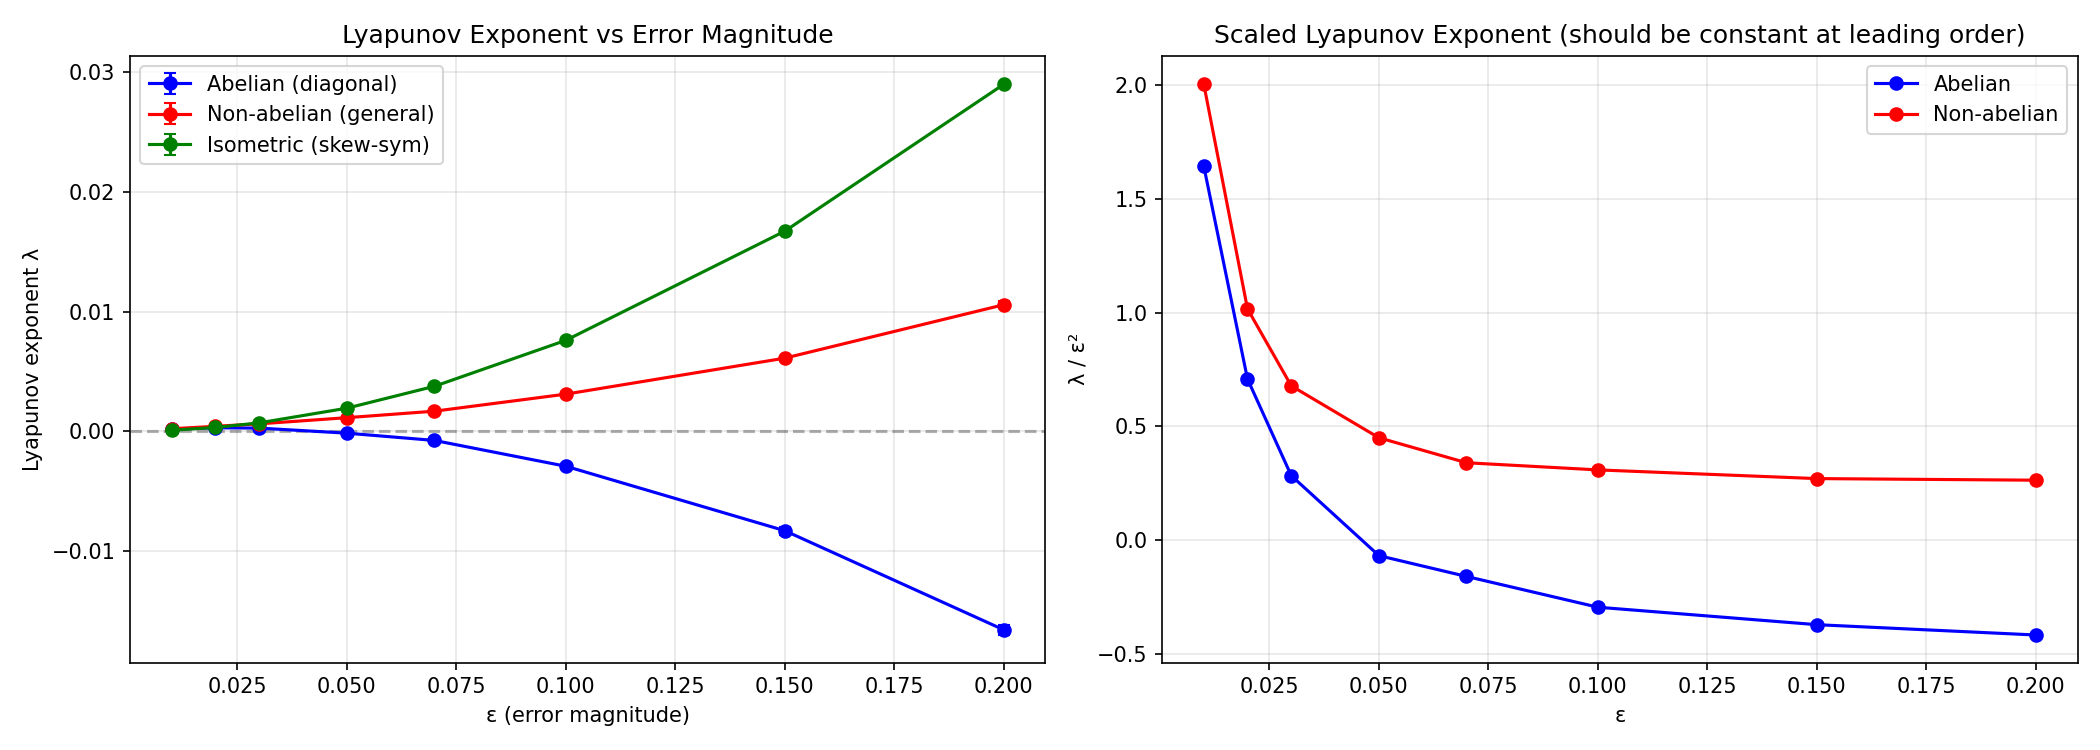
\includegraphics[width=0.85\linewidth]{../results/plots/lyapunov_scaling.png}
\caption{Lyapunov exponent as a function of error magnitude $\eps$
  for diagonal (abelian) and general (non-abelian) error operators
  in $d = 5$ dimensions.  The diagonal exponent becomes negative for
  $\eps \ge 0.05$, confirming contraction, while the general exponent
  remains positive, confirming growth.  This illustrates the ordering
  of Theorem~\ref{thm:lyapunov}.}\label{fig:lyapunov}
\end{figure}

\begin{figure}[ht]
\centering
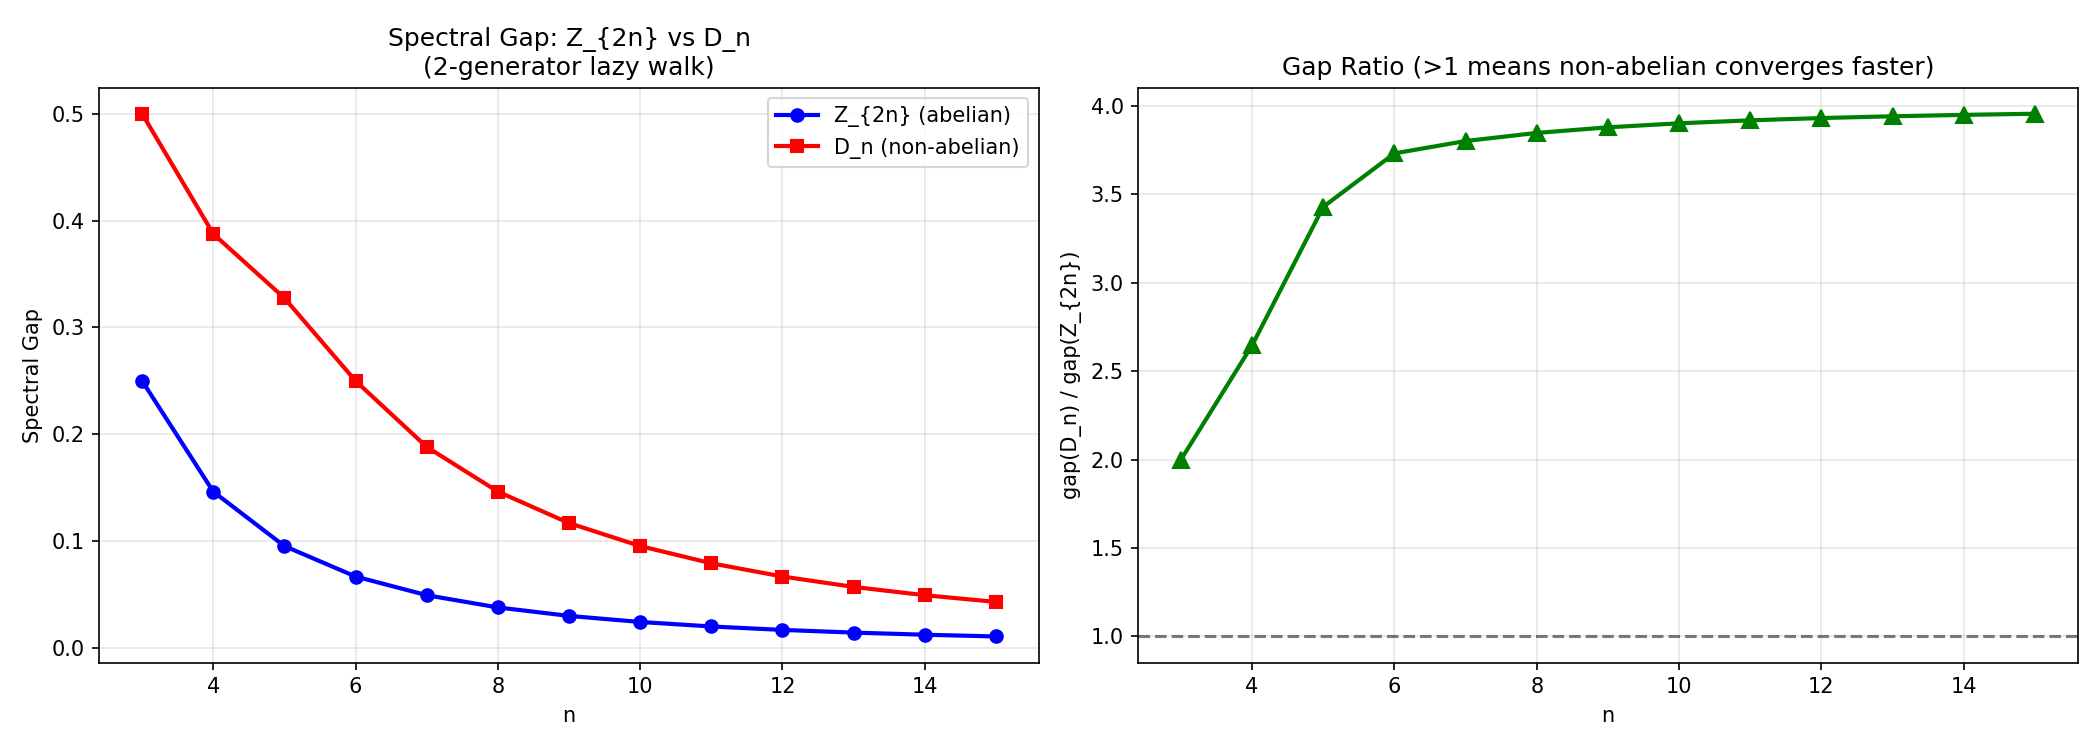
\includegraphics[width=0.85\linewidth]{../results/plots/spectral_gap_comparison.png}
\caption{Spectral gap ratio $\gamma(D_n)/\gamma(\Z_{2n})$ as a
  function of $n$, confirming the convergence to $4$ predicted by
  Theorem~\ref{thm:spectral_gap}\ref{item:ratio}.}\label{fig:spectral}
\end{figure}

\section{Discussion}\label{sec:discussion}

\subsection{Two regimes of commutativity}

Our results reveal a fundamental dichotomy in the role of commutativity
for multi-step proof systems.

\begin{enumerate}[leftmargin=*,itemsep=2pt]
\item \textbf{Error accumulation.}
  Commuting (abelian) error operators yield lower Lyapunov exponents
  (Theorem~\ref{thm:lyapunov}).  This means that when each proof step
  introduces a small perturbation, independent substeps whose errors
  commute produce slower error growth.

\item \textbf{Proof space exploration.}
  Non-abelian groups can have larger spectral gaps
  (Theorem~\ref{thm:spectral_gap}), corresponding to faster mixing of
  the associated random walk.  For proof search, this means that
  non-commuting operations can explore the space of candidate proofs
  more efficiently.
\end{enumerate}

These two objectives---minimizing error accumulation and maximizing
exploration---are fundamentally in tension.  A proof strategy must
balance them: use commuting substeps where errors compound (e.g., in
algebraic simplification chains) and non-commuting operations where
diversity of exploration is needed (e.g., case analysis or induction
strategy selection).

\subsection{Connections to prior work}

\paragraph{Lie group error propagation.}
Theorem~\ref{thm:lyapunov} extends the log-linear error framework
of Barrau and Bonnabel \cite{barrau2014} from continuous-time Lie
group systems to discrete stochastic matrix products.  While
\cite{barrau2014} showed that group-affine systems enjoy linear error
dynamics on the Lie algebra, our result quantifies the Lyapunov
exponent for the discrete setting and shows that the abelian/non-abelian
distinction has concrete consequences for convergence rates.

\paragraph{Quantum error correction.}
The requirement in Gottesman's stabilizer formalism \cite{gottesman1996}
that the stabilizer group be abelian parallels our finding that abelian
error structure yields tighter convergence bounds
(Theorem~\ref{thm:diaconis}).  In both settings, commutativity provides
the algebraic structure needed for systematic error control.
Arvind et al.\ \cite{arvind2002} further showed that abelian subgroups
of the non-abelian error group suffice for constructing error-correcting
codes, analogous to our observation that it is the commutativity of the
error directions (not the full proof transformations) that matters.

\paragraph{Random walks on groups.}
Our Theorem~\ref{thm:spectral_gap} applies the spectral gap framework
of Diaconis \cite{diaconis1988} to the proof search setting.  The
$4{:}1$ asymptotic ratio between the spectral gaps of $D_n$ and
$\Z_{2n}$ illustrates how non-abelian Cayley graphs serve as better
expanders, a phenomenon well-known in the theory of expander graphs
but not previously connected to proof-theoretic convergence.

\paragraph{Error propagation on motion groups.}
Wang and Chirikjian \cite{wang2008} showed that error distributions
on non-abelian Lie groups exhibit coupling between mean and covariance
evolution.  Our commutator-based gap estimate
(Theorem~\ref{thm:lyapunov}\ref{item:gap}) quantifies this coupling
for discrete products and identifies the expected commutator Frobenius
norm as the precise invariant controlling the penalty.

\subsection{Implications for proof systems}

Our results suggest three design principles for iterative proof
refinement systems.

\begin{enumerate}[leftmargin=*,itemsep=2pt]
\item \textbf{Decompose into commuting substeps.}
  When a proof can be decomposed into independent subgoals whose error
  operators commute, error accumulation is minimized
  (Theorem~\ref{thm:lyapunov}\ref{item:diag}).  This favors proof
  strategies based on independent lemmas over tightly coupled reasoning
  chains.

\item \textbf{Use non-commuting operations for search.}
  When the proof strategy involves exploring a space of candidate proofs,
  non-commuting operations (case splits, induction choices) create
  better-connected search graphs (Theorem~\ref{thm:spectral_gap}),
  enabling faster convergence to a correct proof.

\item \textbf{Monitor the commutator norm.}
  The quantity $\E[\frobnorm{\comm{A_1}{A_2}}^2]$ is a computable
  invariant that predicts the convergence penalty from proof step
  interactions (Corollary~\ref{cor:commutator}).  Proof systems could
  estimate this quantity online and adjust their strategy accordingly.
\end{enumerate}

\subsection{Open questions}

We conclude with several directions for future work.

\begin{conjecture}\label{conj:constant}
The dimension-dependent constant $C_d$ in
Theorem~\ref{thm:lyapunov}\ref{item:gap} satisfies
$C_d = \Theta(1)$ as $d \to \infty$, i.e., the Lyapunov gap is
dimension-independent at leading order.  Computational evidence
(Table~\ref{tab:dimension}) supports this.
\end{conjecture}

\begin{table}[ht]
\centering
\caption{Lyapunov exponent gap $\lambda_{\mathrm{gen}} - \lambda_{\mathrm{abel}}$
  as a function of dimension $d$ at $\eps = 0.05$.}\label{tab:dimension}
\begin{tabular}{@{}rc@{}}
\toprule
$d$ & $\lambda_{\mathrm{gen}} - \lambda_{\mathrm{abel}}$ \\
\midrule
2  & 0.000864 \\
4  & 0.001230 \\
6  & 0.001238 \\
8  & 0.001192 \\
10 & 0.001124 \\
\bottomrule
\end{tabular}
\end{table}

\begin{enumerate}[leftmargin=*,itemsep=2pt]
\item \textbf{Discrete proof spaces.}
  Our results use continuous matrix groups.  Extending the framework
  to finite proof state spaces (e.g., propositional proof systems)
  with a purely discrete group structure would make it directly
  applicable to formal verification systems such as Lean or Coq.

\item \textbf{Optimal proof decomposition.}
  Given a proof goal, what is the algorithmically optimal decomposition
  into substeps that minimizes the commutator norm of the resulting
  error operators?  This optimization problem connects our framework
  to proof complexity theory.

\item \textbf{Connection to proof complexity.}
  Can the Lyapunov exponent or spectral gap of the error propagation
  operator be formally related to proof length or proof width in the
  sense of propositional proof complexity?

\item \textbf{Empirical validation.}
  Testing the predictions of Theorems~\ref{thm:lyapunov}
  and~\ref{thm:spectral_gap} on actual proof search traces from
  interactive theorem provers would bridge the gap between our
  theoretical framework and practical proof engineering.
\end{enumerate}

\section{Conclusion}\label{sec:conclusion}

We have established a mathematical framework connecting the algebraic
structure of error propagation to convergence behavior in multi-step
mathematical proofs.  The Lyapunov exponent ordering theorem
(Theorem~\ref{thm:lyapunov}) shows that abelian error operators
accumulate errors strictly more slowly than non-abelian ones, with the
gap controlled by the commutator Frobenius norm at order $\Theta(\eps^2)$.
The spectral gap comparison (Theorem~\ref{thm:spectral_gap}) reveals
that non-abelian groups can mix up to four times faster on matched Cayley
graphs, creating a fundamental tension between error minimization and
exploration efficiency.  The Diaconis bound analysis
(Theorem~\ref{thm:diaconis}) explains why abelian groups yield more
informative convergence bounds.  Together, these results provide a
principled basis for proof strategy design: commuting substeps for error
control, non-commuting operations for search efficiency, and the
commutator norm as a computable diagnostic.

These results bridge Lie group error theory \cite{barrau2014,wang2008,li2023},
quantum error correction \cite{gottesman1996,arvind2002,zhao2023},
and spectral theory of random walks \cite{diaconis1988,furstenberg1963}
into a unified framework applicable to mathematical proof systems.


\bibliographystyle{amsplain}
\bibliography{references}

\end{document}
